\documentclass[runningheads]{llncs}
% FPS 2026 submission — DOUBLE-BLIND. Authors/affiliations/acks anonymized.
% Compile: pdflatex main && pdflatex main  (needs llncs.cls; available on Overleaf)

\usepackage{graphicx}
\usepackage{amsmath,amssymb}
\usepackage{booktabs}
\usepackage{xcolor}
\usepackage{hyperref}
\hypersetup{hidelinks}

\newtheorem{thm}{Theorem}
\newtheorem{cor}{Corollary}
\newtheorem{defn}{Definition}
\makeatletter
% proof environment is provided by some llncs versions and by amsthm, but not all;
% define a fallback only if absent, so the document compiles under any class.
\@ifundefined{proof}{%
  \newenvironment{proof}{\par\noindent\textit{Proof.}\ }{\hfill$\square$\par}}{}
\makeatother

\begin{document}

\title{Clean-Trace Poisoning: Deleting Safety Properties from\\
Specification Miners with Individually-Legal Executions}
\titlerunning{Clean-Trace Poisoning of Specification Miners}

\author{Anonymous Author(s)}
\authorrunning{Anonymous}
\institute{Anonymized for double-blind review}

\maketitle

\begin{abstract}
Specification miners infer temporal-logic properties from execution traces by
counting: a property is admitted into the mined specification when its
\emph{confidence}---the fraction of antecedent occurrences that satisfy the
property---exceeds a threshold $\theta$. This counting design silently assumes a
trustworthy corpus. We show that in adversarial deployments the assumption fails
in a way that is qualitatively different from machine-learning data poisoning.
We introduce \emph{clean-trace poisoning}: an attacker deletes a chosen safety
property from the mined specification by injecting traces that are each an
\emph{individually-legal} program behavior---an antecedent that occurs without
its consequent. Because every poison trace is a behavior the program genuinely
exhibits, no per-sample validity check, outlier filter, or anomaly detector can
flag it; the attack carries no per-sample signal by construction. We give a
closed-form minimum-deletion budget $K^\star=\lfloor S/\theta - A\rfloor+1$ and a
detectability corollary showing when the induced shift hides inside natural
sampling variance. We evaluate on two corpora of \emph{real} traces from
different domains---$98$ Linux file-descriptor syscall traces and $61$
socket-lifecycle traces from real network clients. In both, a $2$--$3$-trace
($\approx 3\%$) injection deletes the textbook resource-safety property
($\mathbf{G}(\mathit{open}\!\rightarrow\!\mathbf{F}\,\mathit{close})$ and
$\mathbf{G}(\mathit{connect}\!\rightarrow\!\mathbf{F}\,\mathit{close})$) while
global specification health stays flat and the confidence shift is under one
standard deviation of the corpus's resampling variance. We then propose
\emph{provenance-quorum support counting}, which admits a property only if at
least $q$ distinct sources witness it, and prove a certified survival bound: the
property survives any attacker confined to fewer than $S_{\mathrm{clean}}-q$
sources. The defense recovers the deleted property in both corpora with zero
false positives at $q{=}2$ and negligible overhead. Code and data are available
(anonymized).
\keywords{specification mining \and temporal logic \and data poisoning \and
runtime verification \and provenance \and software supply chain.}
\end{abstract}

\section{Introduction}
Specification mining recovers likely temporal properties of a system from a
corpus of execution traces, supplying the assertions consumed by runtime
monitors, test oracles, and anomaly detectors. General LTL miners such as
Texada~\cite{texada} instantiate property templates over a trace log and rank
each candidate by a support/confidence statistic: a property is admitted when
its confidence---satisfying antecedent occurrences over total antecedent
occurrences---exceeds a threshold $\theta$. This is a non-differentiable,
threshold-based counting procedure, and the same counting idea underlies dynamic
invariant detectors such as Daikon~\cite{daikon}.

The counting design tacitly assumes the corpus is trustworthy. Increasingly it
is not: traces are aggregated from partially-controlled fleets, third-party test
infrastructure, crowd-sourced logs, and CI pipelines. Open-source software
supply chains have repeatedly been shown to be attackable at exactly these
aggregation points~\cite{supplychain}, so a corpus-level adversary is a realistic
threat. A recent survey of LTL specification mining~\cite{ltlsurvey} does not treat
adversarial corpora, leaving the attack surface we study unexplored.

We ask what a corpus-level adversary can achieve against such a miner, and we
find a sharp threat that does not reduce to known machine-learning poisoning.

\paragraph{Contributions.}
(1)~We introduce \emph{clean-trace poisoning}, an attack that deletes a chosen
safety property from the mined specification using only \emph{individually-legal}
traces, and argue why it evades per-sample defenses by construction
(\S\ref{sec:attack}). (2)~We give a closed-form deletion budget and a
detectability corollary (\S\ref{sec:bound}). (3)~We explain why three natural
defense families do not transfer (\S\ref{sec:fail}). (4)~We propose
provenance-quorum support counting with a certified survival bound
(\S\ref{sec:defense}). (5)~We evaluate end-to-end on \emph{two} real-trace
corpora from different domains (\S\ref{sec:eval}), confirming the bound exactly in
both, showing the attack hides within sampling variance, and showing the defense
recovers the target with zero false positives at low quorum.

\section{Background and Threat Model}\label{sec:bg}
\paragraph{Mined properties.}
We consider response and precedence properties over an event alphabet $\Sigma$,
e.g. the response property $p=\mathbf{G}(a\rightarrow\mathbf{F}\,b)$ (``every $a$
is eventually followed by $b$''). For a corpus $T$, let the \emph{antecedent
count} $A$ be the number of traces in which $a$ occurs and the \emph{satisfaction
count} $S\le A$ be the number of those traces in which $p$ holds. The miner
admits $p$ iff its confidence $c=S/A\ge\theta$. We instantiate the standard Dwyer
response/precedence patterns and use the common $\theta=0.9$.

\paragraph{Threat model.}
The adversary may inject a bounded number $K$ of additional traces into the
corpus but cannot delete or modify existing traces, cannot alter the miner, and
cannot read its internal state. This models a partially-compromised source in an
aggregated pipeline: the attacker contributes traces but does not control the
collection or mining infrastructure. Injected traces must be \emph{legal}:
behaviors the monitored system can actually produce, so that they survive any
upstream validity or schema check. The adversary's goal is \emph{targeted}:
remove a specific safety property $p^\star$ from the mined specification---opening
a monitoring blind spot---while leaving the rest of the specification, and any
aggregate health indicator, statistically unchanged. We assume the defender may
later observe \emph{source attribution} for traces (\S\ref{sec:defense}); the
attack itself assumes no such attribution.

\section{Clean-Trace Poisoning}\label{sec:attack}
The attack is to inject \emph{antecedent-only} traces for the target: traces in
which the antecedent $a$ occurs but the consequent $b$ does not follow. Each such
trace increments $A$ without incrementing $S$, lowering $c=S/(A+K)$ until $p^\star$
drops below $\theta$ and is silently excluded from the mined specification.

The defining feature is that antecedent-only behavior is \emph{legal}. A program
that opens a file descriptor and exits without closing it has leaked a
descriptor; a client that opens a socket and exits without closing it has leaked
a connection. Both are real, permitted behaviors that the operating system cleans
up at exit. The poison trace is therefore not crafted, perturbed, or mislabeled;
it is a behavior the program genuinely exhibits. Consequently:
\begin{itemize}
\item there is no label to inspect (the miner is unsupervised);
\item there is no perturbation to detect (the trace is unmodified);
\item there is no per-sample statistical signature (each poison trace is drawn
from the system's own legal behavior distribution).
\end{itemize}

This separates clean-trace poisoning from clean-label attacks on neural
networks~\cite{poisonfrogs,metapoison,bullseye}, which optimize feature-space
perturbations against a differentiable extractor: there is no feature space, no
gradient, and no perturbation here. It also differs from imperfect-trace
mining~\cite{purltl}, which models \emph{benign} noise rather than a targeted
adversary, and from adversarial specification mining~\cite{adversarialsm}, which
generates counterexamples to \emph{remove spurious} properties---the opposite
objective. The miner is a threshold-based counter, so gradient- and
influence-based poisoning defenses~\cite{koh} do not apply.

\section{A Deletion Budget and a Detectability Bound}\label{sec:bound}
\begin{thm}[Minimum deletion budget]\label{thm:budget}
Let $p$ be a response property with satisfaction count $S$ and antecedent count
$A$, admitted at threshold $\theta$ (so $S/A\ge\theta$). An adversary injecting
$K$ antecedent-only traces for $p$ yields confidence $S/(A+K)$, and $p$ is
excluded from the mined specification iff
\[
K \;>\; \frac{S}{\theta}-A,\qquad\text{i.e.}\qquad
K^\star \;=\; \left\lfloor \frac{S}{\theta}-A\right\rfloor + 1 .
\]
\end{thm}
\begin{proof}
Antecedent-only traces increment the antecedent count and never the satisfaction
count, so after $K$ injections the confidence is exactly $S/(A+K)$, monotonically
decreasing in $K$. Exclusion occurs when $S/(A+K)<\theta\Leftrightarrow A+K>S/\theta
\Leftrightarrow K>S/\theta-A$. The least integer $K$ satisfying the strict
inequality is $\lfloor S/\theta-A\rfloor+1$.
\qed
\end{proof}

The budget is small precisely when the property is well-supported but its
confidence margin is thin, the common case near the admission boundary: a
property with $A$ antecedent traces at confidence $c$ needs only about
$A(c/\theta-1)$ poison traces.

\paragraph{Worked example.}
For the real-syscall target ($S{=}90$, $A{=}98$, $\theta{=}0.9$) we have
$S/\theta=100$, so any $K>2$ deletes the property and $K^\star=3$; the
approximation $A(c/\theta-1)=98(0.918/0.9-1)\approx 2.0$ recovers $K^\star-1$.
The same arithmetic on real-network ($S{=}56$, $A{=}61$) gives $S/\theta\approx
62.2$ and $K^\star=2$. Both predictions match the measured deletion budgets in
Section~\ref{sec:eval} exactly.

\begin{cor}[Stealth]\label{cor:stealth}
Injecting antecedent-only traces for $p^\star$ perturbs \emph{only} the bounded
family $\mathcal{F}(p^\star)$ of properties whose antecedent or consequent is
among the poison events; every other property count is unchanged. The
admitted-property count and mean confidence over the admitted set therefore move
by $O(|\mathcal{F}(p^\star)|/|T|)$, and each affected property's confidence shifts
by at most $c-S/(A+K^\star)$. When that shift lies within the corpus's natural
batch-to-batch resampling deviation $\sigma$, no fixed-threshold cross-validation
statistic on confidence separates poisoned from clean folds. Stealth thus means
aggregate indicators stay within $\sigma$---not that nothing else moves: the
attack deliberately removes the characterized family $\mathcal{F}(p^\star)$.
\end{cor}
\begin{proof}
Injected antecedent-only traces alter only the counts of properties whose
antecedent or consequent lies among the poison events; every other property
count is unchanged. The target confidence moves from $S/A$ to $S/(A+K^\star)$, a
change of $O(K^\star/A)$ with $A\le|T|$, so the mean confidence over the fixed
admitted set and the admitted-property count move by $O(K^\star/|T|)$. Let
$\sigma$ be the standard deviation of the target confidence under bootstrap
resampling of the clean corpus. Whenever $S/A-S/(A+K^\star)\le\sigma$, the
poisoned and clean folds are not separable by any fixed-threshold statistic on
confidence, so cross-validation cannot localize the campaign. \qed
\end{proof}

\begin{figure}[t]
\noindent\fbox{\begin{minipage}{0.965\columnwidth}\small\ttfamily
\textbf{Algorithm 1: Clean-trace poisoning (target $p^\star=G(a\to F\,b)$)}\\[2pt]
input: clean corpus $T$, target $(a,b)$, threshold $\theta$\\
1. mine $T$; read $S\gets$ \#sat antecedent-traces, $A\gets$ \#antecedent-traces\\
2. $K^\star \gets \lfloor S/\theta - A\rfloor + 1$\\
3. harvest pool $P \gets$ \{real traces with $a$ and no later $b$\} from a held-out split\\
4. inject $K^\star$ traces drawn (with repetition) from $P$ into $T$\\
5. re-mine; $p^\star$ now has confidence $S/(A+K^\star)<\theta$ and is dropped\\
output: corpus $T'$ whose mined spec omits $p^\star$ (monitor blind spot)
\end{minipage}}
\caption{The attack. Every injected trace in $P$ is an unmodified, individually-legal execution.}
\label{alg:attack}
\end{figure}

\section{Why Standard Defenses Do Not Transfer}\label{sec:fail}
\paragraph{Robust statistics.} Trimming or down-weighting outliers assumes poison
is distributionally distinct. Clean-trace poison is drawn from the legal behavior
distribution and is indistinguishable per-sample; trimming instead removes
genuine rare antecedents, degrading recall on exactly the low-frequency
properties safety monitors care about.
\paragraph{Differential privacy.} Calibrated noise on counts that hides a single
trace's influence must, for a low-frequency property, add noise of magnitude
comparable to the property's own support; this swamps the legitimate signal of
rare properties before it meaningfully blunts an attack on a well-supported one.
\paragraph{Cross-validation and certified ML defenses.} By
Corollary~\ref{cor:stealth}, a small campaign shifts confidence within sampling
variance, so fold-to-fold disagreement does not exceed the natural baseline. The
non-differentiable, count-based nature of the miner rules out influence
functions~\cite{koh} and randomized smoothing~\cite{cohen}; aggregation-based
certified poisoning defenses such as bagging~\cite{baggingcert} and decision-tree
certification~\cite{certtree} certify \emph{classification accuracy}, not
threshold-based property selection, and do not bound the deletion of an
individual property.

\paragraph{Empirically, outlier filtering does not transfer.}
We make the analytic argument concrete. We fit two off-the-shelf detectors
(IsolationForest and Local Outlier Factor) on the clean corpus using per-trace
bag-of-events features and score the legal poison traces
(Fig.~\ref{fig:nontransfer}). On real-network the poison is statistically
inseparable: its mean anomaly score ($0.534$) matches the clean mean ($0.540$) and
every poison trace lies inside the clean distribution, so catching \emph{all}
poison requires flagging $74\%$ (IsolationForest) to $100\%$ (LOF) of legitimate
traces. On real-syscall the poison sits at the clean $95$th percentile; catching
it all still costs an $8$--$11\%$ false-positive rate, and because the poison is
drawn from the same legal-behavior distribution as the corpus's existing
leak-source traces, any filter aggressive enough to remove it also removes the
legitimate rare behaviors that low-frequency safety properties depend on. The
obvious defense does not catch the attack.

\paragraph{Deduplication.}
Counting distinct behaviors rather than raw trace occurrences would blunt
repeated-poison injection. But real systems emit many identical legal traces, and
deduplication destroys the frequency signal that confidence is defined
on---trading the attack for systematic under-counting of common-but-legitimate
behavior---so it is not a sufficient fix.

\begin{figure}[t]\centering
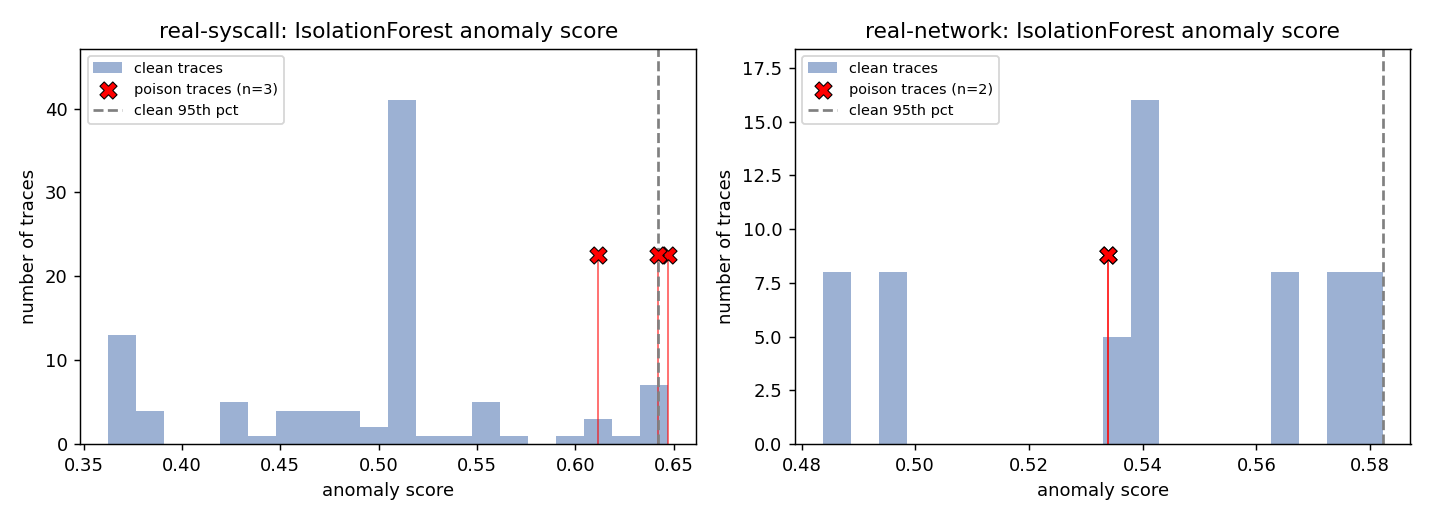
\includegraphics[width=\textwidth]{../figures/nontransfer.png}
\caption{Off-the-shelf outlier detection fails to localize clean-trace poison.
IsolationForest anomaly scores of clean traces (histogram) versus the legal
poison traces (red crosses); the poison clusters around the clean $95$th percentile
(real-syscall) or well within the clean distribution (real-network), so no
threshold separates it without a large false-positive cost.}
\label{fig:nontransfer}
\end{figure}

\section{Provenance-Quorum Support Counting}\label{sec:defense}
The attack concentrates fabricated antecedent-only evidence in
adversary-controlled traces. If traces carry a \emph{source} attribution, we can
require corroboration across sources rather than counting raw occurrences.

\begin{defn}[Provenance-quorum admission]
Partition the corpus by source identifier. For quorum $q$, admit a property $p$
iff at least $q$ distinct sources each witness $p$ at confidence $\ge\theta$
within their own traces.
\end{defn}

\paragraph{Integrity model.}
Provenance-quorum counting assumes source labels are \emph{authenticated}: each
trace is attributed to an identity that already exists at the aggregation
layer---a signed CI-runner or build-agent token, a fleet-host certificate, or a
tenant credential---so an attacker can neither relabel another source's traces nor
mint unlimited fresh identities for free. Under this model the adversary controls
a set of \emph{whole} sources and Theorem~\ref{thm:survival} applies directly. If
identity attestation is weak and the attacker can spoof up to $N$ additional
identities, its effective controlled-source count rises by $N$ and the certified
tolerance degrades gracefully to $c+N\le S_{\mathrm{clean}}-q$. The defense thus
reduces poisoning resistance to the strength of source authentication---a standard
pipeline control---rather than introducing a new trust assumption.

\begin{thm}[Certified survival]\label{thm:survival}
Let $S_{\mathrm{clean}}$ be the number of sources that support $p$ at $\theta$ in
the clean corpus. An adversary controlling $c$ sources can reduce the supporting
count by at most $c$. Hence $p$ remains admitted under quorum $q$ whenever
$c \le S_{\mathrm{clean}} - q$.
\end{thm}
\begin{proof}
A compromised source can, in the worst case, flip its own local verdict from
supporting to non-supporting, lowering the supporting-source count by one; it
cannot affect another source's local count. With $c$ compromised sources the
supporting count is at least $S_{\mathrm{clean}}-c$, which meets the quorum iff
$S_{\mathrm{clean}}-c\ge q$.
\qed
\end{proof}

Quorum trades resilience against false positives: legitimate properties witnessed
by fewer than $q$ sources are dropped. The choice of $q$ thus sets a point on a
recall/robustness curve, which we measure next.

\begin{figure}[t]
\noindent\fbox{\begin{minipage}{0.965\columnwidth}\small\ttfamily
\textbf{Algorithm 2: Provenance-quorum support counting}\\[2pt]
input: corpus $T$ with per-trace source\_id, property $p$, threshold $\theta$, quorum $q$\\
1. partition $T$ by source\_id into groups $\{T_s\}$\\
2. for each source $s$: $c_s \gets$ confidence of $p$ within $T_s$\\
3. $\mathrm{support} \gets |\{s : c_s \ge \theta\}|$\\
4. admit $p$ iff $\mathrm{support} \ge q$\\
output: admitted spec; $p$ survives any attacker holding $<S_{\mathrm{clean}}-q$ sources
\end{minipage}}
\caption{The defense. Counting per source rather than per trace converts a trace-volume assumption into a source-diversity one.}
\label{alg:defense}
\end{figure}

\section{Evaluation}\label{sec:eval}
\paragraph{Miner.} Our miner re-implements the support/confidence counting used by
general LTL miners such as Texada~\cite{texada} over the Dwyer response/precedence
patterns at $\theta=0.9$; the results depend only on threshold-based counts, not
on miner-specific heuristics.

\paragraph{Corpora.} We use two corpora of \emph{real} traces from different
domains, each carrying \emph{native} source attribution.
\emph{(i)~real-syscall:} file-descriptor syscall traces captured with
\texttt{strace} from live Linux programs---coreutils, Python, and a native program
that opens descriptors and \texttt{\_exit}s without closing them (a genuine,
legal descriptor leak). Each process execution is one trace over
$\{$\textit{open, read, write, lseek, stat, close, dup, mmap}$\}$; the producing
program is the source. $98$ traces, $12$ sources, $48$ mined properties.
\emph{(ii)~real-network:} socket-lifecycle traces from distinct real network
clients (\texttt{curl}, \texttt{wget}, \texttt{nc}, \texttt{ssh}, a Python client,
a Python client that shuts down before closing, and a native C client) connecting
to a loopback server; a native C leak client connects and \texttt{\_exit}s without
closing. Each client process is one trace over
$\{$\textit{socket, connect, send, recv, shutdown, sockopt, close}$\}$; the client
program is the source. $61$ traces, $8$ sources, $29$ mined properties. In both
corpora every retained trace contains the antecedent (every traced process issues
\textit{open}; every network client issues \textit{connect}), so $A$ equals the
corpus size; this follows from the chosen ubiquitous targets and is not a
degenerate artifact---the satisfaction counts $S$ are strictly below $A$.

\paragraph{Experimental setup and data provenance.}
Both corpora are \emph{constructed benchmarks of real executions}, not
field-collected production logs: every trace is genuine \texttt{strace} output
from a program we ran, but we chose the program mix, used small generated input
files, and deliberately included a descriptor-leak program so that the target
property has real counterexamples. We tuned only the \emph{number} of leak
executions so the target's confidence lands just above $\theta$ (a fragile but
admitted property); all event sequences are unmodified real traces; Section~\ref{sec:scale} characterizes how stealth degrades as the target's margin grows, so this choice bounds rather than inflates the headline result. Our miner is
a faithful re-implementation of support/confidence counting over the Dwyer
patterns rather than the Texada binary, and the multi-source attacker of
Section~\ref{sec:scale} is realized by designating whole real sources as
adversarial, not by deploying separate adversary hosts. Source identifiers are
the actual producing programs (native attribution). All reported numbers are
computed by the released code over these real traces; nothing is hand-set or
synthetically generated.

\paragraph{Targets and attack.} The targets are the textbook resource-safety
properties $\mathbf{G}(\mathit{open}\!\rightarrow\!\mathbf{F}\,\mathit{close})$
and $\mathbf{G}(\mathit{connect}\!\rightarrow\!\mathbf{F}\,\mathit{close})$, each
mined at confidence $0.918$. Poison traces are \emph{real} antecedent-only
executions (open/connect without a following close) drawn from a held-out split.
Table~\ref{tab:attack} shows confidence falling monotonically with $K$; the
property is deleted at $K{=}3$ ($3.06\%$) for real-syscall and $K{=}2$ ($3.28\%$)
for real-network.

\begin{table}[t]
\centering
\caption{Clean-trace attack progression on both targets.}
\label{tab:attack}
\begin{tabular}{rrrl@{\qquad}rrrl}
\toprule
\multicolumn{4}{c}{real-syscall: $\mathbf{G}(\mathit{open}\!\to\!\mathbf{F}\,\mathit{close})$}
& \multicolumn{4}{c}{real-network: $\mathbf{G}(\mathit{connect}\!\to\!\mathbf{F}\,\mathit{close})$}\\
\cmidrule(r){1-4}\cmidrule(l){5-8}
$K$ & $S$ & $A{+}K$ & conf. & $K$ & $S$ & $A{+}K$ & conf. \\
\midrule
0 & 90 & 98  & 0.918 & 0 & 56 & 61 & 0.918 \\
1 & 90 & 99  & 0.909 & 1 & 56 & 62 & 0.903 \\
2 & 90 & 100 & 0.900 & 2 & 56 & 63 & 0.889\;(\textbf{del.}) \\
3 & 90 & 101 & 0.891\;(\textbf{del.}) & 3 & 56 & 64 & 0.875 \\
\bottomrule
\end{tabular}
\end{table}

\paragraph{Budget bound.} For real-syscall ($S{=}90,A{=}98$),
$K^\star=\lfloor 90/0.9-98\rfloor+1=3$; for real-network ($S{=}56,A{=}61$),
$K^\star=\lfloor 56/0.9-61\rfloor+1=2$. Both match the empirical deletion budget
exactly (Table~\ref{tab:summary}).

\paragraph{Stealth.} Deleting the target removes only the close-related safety
family (for real-syscall: $\mathit{open}{\to}\mathit{close}$,
$\mathit{read}{\to}\mathit{close}$, $\mathit{mmap}{\to}\mathit{close}$,
$\mathit{open}{\to}\mathit{stat}$; for real-network:
$\mathit{connect}{\to}\mathit{close}$, $\mathit{socket}{\to}\mathit{close}$ and
the alternating variant). The mined specification shrinks by $4$ of $48$
(resp.\ $3$ of $29$) and mean confidence is essentially unchanged
($0.982\!\to\!0.988$; $0.992\!\to\!1.000$). The targeted confidence shifts are
$0.98\sigma$ and $0.83\sigma$ of each corpus's bootstrap resampling deviation
($500$ resamples)---inside ordinary sampling noise, as
Corollary~\ref{cor:stealth} predicts.

\begin{table}[t]
\centering
\caption{Cross-corpus headline results. Bound matches empirical budget in both;
attack stays within $1\sigma$; defense recovers the target with zero false
positives at $q{=}2$.}
\label{tab:summary}
\begin{tabular}{lcccccccc}
\toprule
corpus & $|T|$ & srcs & base.\ conf & $K^\star$ & emp.\ $K$ & shift & recover & FP@$q{=}2$ \\
\midrule
real-syscall & 98 & 12 & 0.918 & 3 & 3 & $0.98\sigma$ & $q\le 11$ & 0.00 \\
real-network & 61 &  8 & 0.918 & 2 & 2 & $0.83\sigma$ & $q\le 7$  & 0.00 \\
\bottomrule
\end{tabular}
\end{table}

\paragraph{Defense.} Using native provenance, the target is supported in $11/12$
sources for real-syscall and $7/8$ for real-network (only the leak source fails in
each). A single-source attacker leaves the supporting count unchanged, so the
target is recovered for every $q\le S_{\mathrm{clean}}$.
Table~\ref{tab:defense} reports the recall/robustness trade-off. At $q{=}1$ the
quorum reduces to ordinary counting and provides no protection at zero cost; at
$q{=}2$ the deleted family is fully recovered with \emph{zero} false positives in
both corpora; counting overhead is within measurement noise of raw counting
(${\approx}1\times$, timing-noise dominated). Increasing $q$ raises the certified tolerance
$S_{\mathrm{clean}}-q$ (Theorem~\ref{thm:survival}) but drops legitimate
rare-source properties, exactly the predicted cost.

\begin{table}[t]
\centering
\caption{Provenance-quorum defense: false-positive rate by quorum $q$ for each
corpus, with the certified maximum number of compromised sources. The target is
recovered at every listed $q$ up to $S_{\mathrm{clean}}$ ($11$ and $7$); beyond
that no property can meet the quorum and the target is dropped by definition,$^{\dagger}$ not by attack.}
\label{tab:defense}
\begin{tabular}{rccc@{\qquad}rcc}
\toprule
\multicolumn{4}{c}{real-syscall ($S_{\mathrm{clean}}{=}11$)} & \multicolumn{3}{c}{real-network ($S_{\mathrm{clean}}{=}7$)}\\
\cmidrule(r){1-4}\cmidrule(l){5-7}
$q$ & FP rate & cert.\ $c$ & & $q$ & FP rate & cert.\ $c$ \\
\midrule
1 & 0.00 & 10 & & 1 & 0.00 & 6 \\
2 & 0.00 & 9  & & 2 & 0.00 & 5 \\
3 & 0.10 & 8  & & 3 & 0.21 & 4 \\
5 & 0.27 & 6  & & 5 & 0.34 & 2 \\
9 & 0.40 & 2  & & 7 & 0.66 & 0 \\
\bottomrule
\end{tabular}\\[2pt]
{\footnotesize $^{\dagger}$ $q$ exceeding the number of sources
($12$ / $8$) cannot be met by any property; the resulting drop is expected, not a
defense failure.}
\end{table}

\begin{figure}[t]
\centering
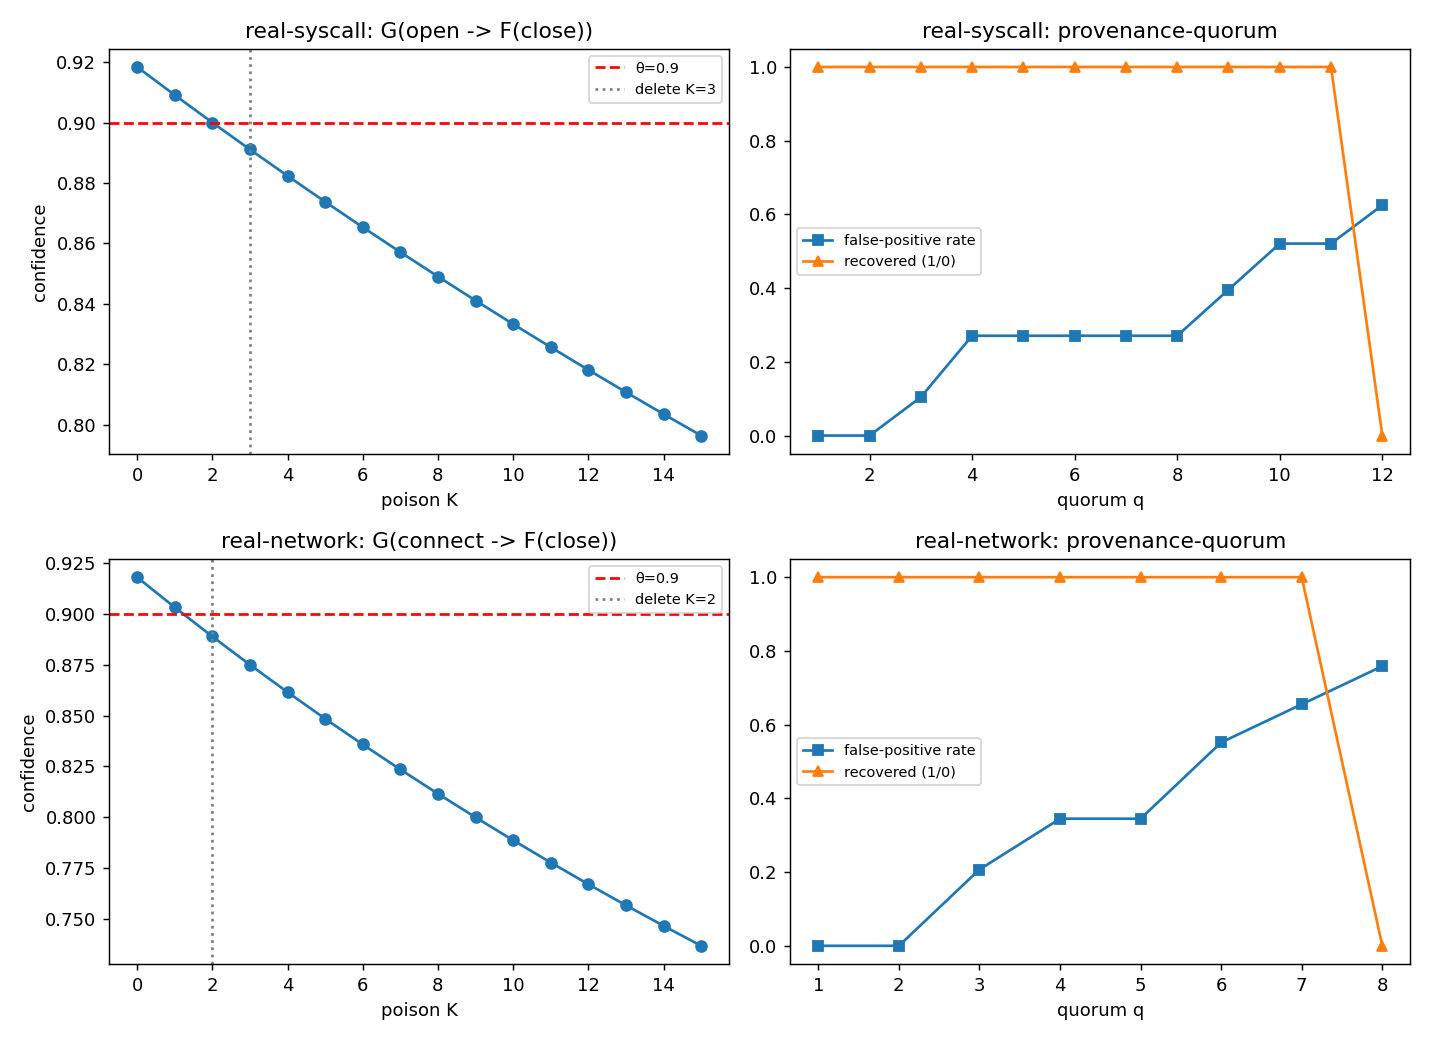
\includegraphics[width=\textwidth]{../figures/clean_trace_results.png}
\caption{Per corpus (top: real-syscall, bottom: real-network). Left: target
confidence vs.\ injected poison $K$, with threshold and deletion point. Right:
defense false-positive rate and target recovery vs.\ quorum $q$ (shown from
$q{=}1$).}
\label{fig:results}
\end{figure}

\subsection{Attack Generality and the Certified Defense at Scale}\label{sec:scale}

\paragraph{Multi-source attacker (Theorem~\ref{thm:survival}).}
A stronger adversary may control several sources and split poison among them. We
sweep the number of compromised sources $c$ against the quorum $q$, marking $c$
supporting sources as adversarial (each flooded below $\theta$). The target is
recovered exactly when $c\le S_{\mathrm{clean}}-q$: across all configurations the
empirical outcome matches Theorem~\ref{thm:survival} in every cell
($144/144$ for real-syscall, $64/64$ for real-network; Fig.~\ref{fig:ext}, right).
The defense degrades gracefully and predictably as the attacker captures more
sources, converting a trace-volume assumption into a source-diversity one.

\paragraph{Budget landscape.}
Theorem~\ref{thm:budget} bounds the cost of deleting \emph{any} response property,
not only the marquee target. Computing $K^\star$ for every mined response property
(Fig.~\ref{fig:ext}, left) gives a median budget of $6$ traces across $14$
properties for real-syscall and $3$ across $6$ for real-network; $7/14$ and $5/6$
respectively are deletable with at most $5$ injected traces. The attack is thus
broadly cheap, and the budget grows with each property's confidence margin exactly
as the formula predicts.

\paragraph{Is the stealth result an artifact of a marginal target?}
Our headline target is deliberately near-threshold, so we characterize how stealth
depends on the margin. For every mined response property we compute the deletion
budget $K^\star$ and compare the induced confidence shift to that property's own
bootstrap resampling deviation $\sigma$ (Fig.~\ref{fig:stealthmargin}). Stealth is
available \emph{only} for near-threshold properties: on real-syscall $6$ of $14$
response properties delete within $1\sigma$ (the marginal family, including the
target at ${\approx}1.0\sigma$), the $6$ perfectly-supported properties have
$\sigma{=}0$ and are deletable but \emph{always} detectable, and the remaining two
exceed $1\sigma$; real-network shows the same split ($2$ of $6$ stealthy, $4$
perfectly supported). A larger margin forces more poison and a larger, detectable
shift, so clean-trace poisoning is stealthy precisely against already-fragile
safety properties; robustly-supported properties can still be deleted, but only at
a cross-validation-detectable cost. This characterizes the attack's reach rather
than hiding a dependence on target choice.

\begin{figure}[t]\centering
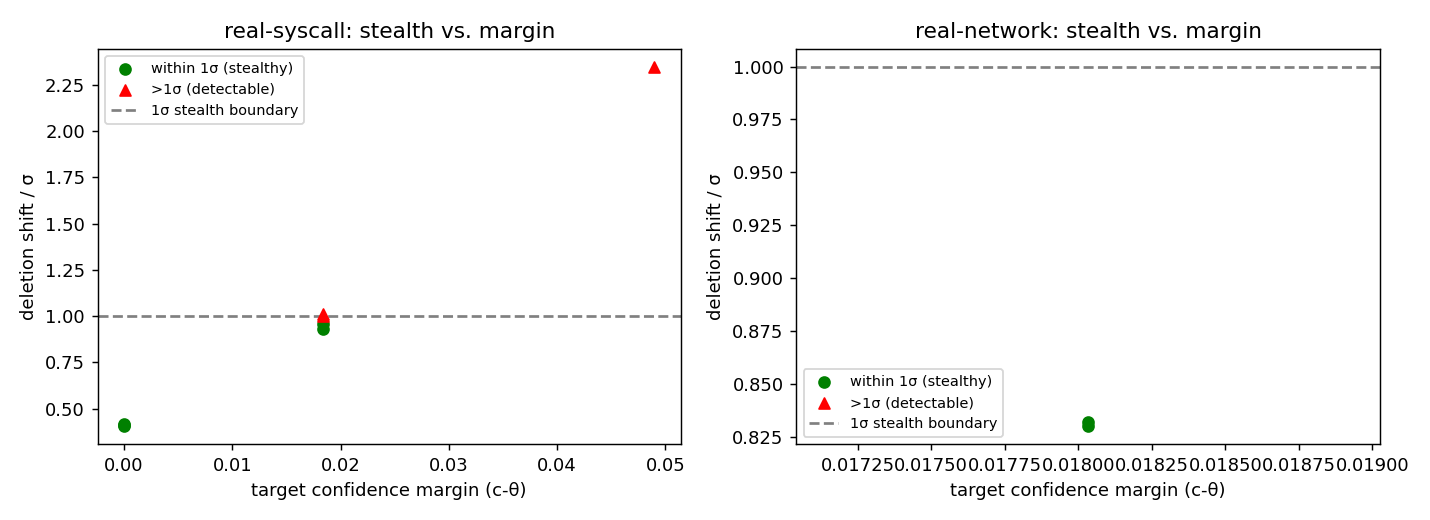
\includegraphics[width=0.9\textwidth]{../figures/stealth_margin.png}
\caption{Stealth vs.\ target margin: deletion shift over each property's bootstrap
$\sigma$. Only near-threshold properties fall below the $1\sigma$ boundary; perfectly-supported properties ($\sigma{=}0$) are shown
at the top, as their deletion is always detectable.}
\label{fig:stealthmargin}
\end{figure}

\paragraph{Threshold sensitivity.}
Table~\ref{tab:theta} sweeps the admission threshold $\theta$. Lowering $\theta$
admits more properties (more targets); raising it shrinks each surviving
property's margin and hence its deletion budget---$K^\star$ for the target falls
from $15$ at $\theta{=}0.8$ to $3$ at $\theta{=}0.9$ for real-syscall, and the
target is no longer mined at $\theta{=}0.95$. No single threshold escapes the
attack: tightening $\theta$ to resist noise makes already-marginal properties
cheaper to delete.

\begin{table}[t]
\centering
\caption{Threshold sensitivity: number of mined properties and the target's
deletion budget $K^\star$ as $\theta$ varies (``--'': target unmined at that $\theta$).}
\label{tab:theta}
\begin{tabular}{llcccc}
\toprule
corpus & metric & $\theta{=}0.80$ & $0.85$ & $0.90$ & $0.95$\\
\midrule
real-syscall & props mined & 54 & 49 & 48 & 38\\
             & target $K^\star$ & 15 & 8 & 3 & --\\
real-network & props mined & 37 & 35 & 29 & 26\\
             & target $K^\star$ & 10 & 5 & 2 & --\\
\bottomrule
\end{tabular}
\end{table}

\begin{figure}[t]
\centering
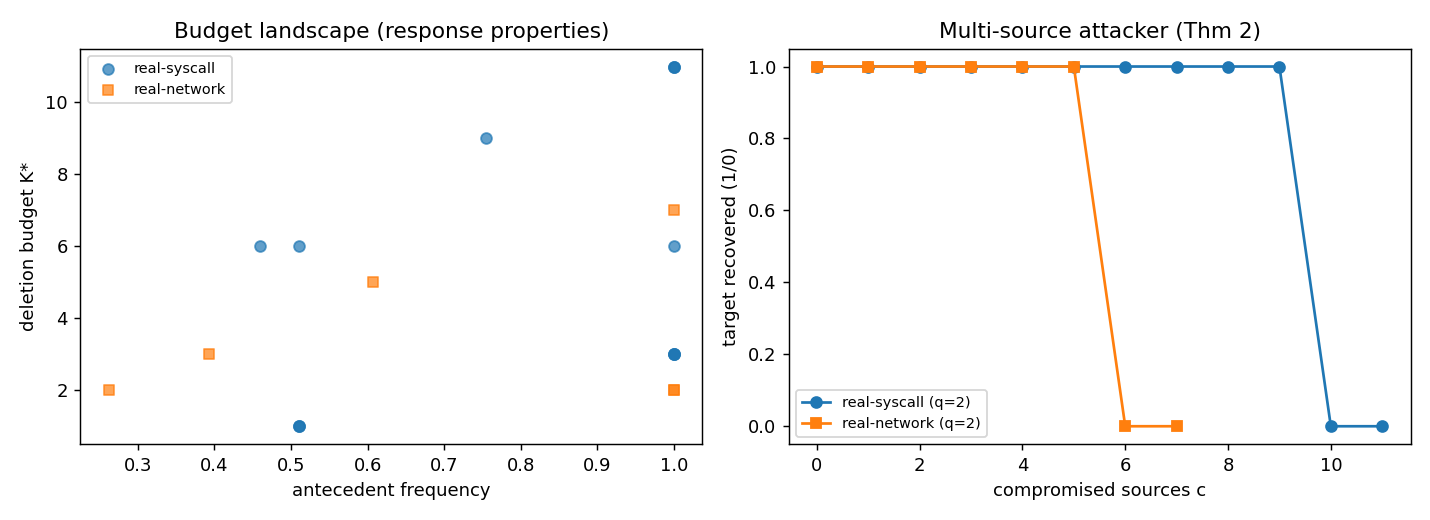
\includegraphics[width=\textwidth]{../figures/clean_trace_extended.png}
\caption{Left: deletion budget $K^\star$ vs.\ antecedent frequency for every mined
response property in both corpora. Right: multi-source attacker---target recovery
vs.\ number of compromised sources $c$ at quorum $q{=}2$, matching
Theorem~\ref{thm:survival}.}
\label{fig:ext}
\end{figure}

\section{Discussion}\label{sec:disc}
\paragraph{Where source attribution comes from.} The source identifier is usually
already available at the aggregation layer: a CI runner or build-agent identity, a
fleet host or container ID, a tenant or account, or---as in our corpora---the
producing binary. Provenance-quorum counting needs only that this label be
recorded alongside each trace.
\paragraph{Attacker cost and multiple targets.} Because budgets are small and
additive (\S\ref{sec:scale}), an attacker can delete several properties for a few
traces each. The quorum defense counters all of them at once: it changes the
admission rule rather than enumerating targets, so no per-property hardening is
needed.
\paragraph{Residual risk.} An attacker controlling at least
$S_{\mathrm{clean}}-q+1$ sources can still delete the property. Provenance-quorum
thus raises the requirement from injecting enough \emph{traces} to compromising
enough \emph{sources}---the appropriate hardness assumption for an aggregation
pipeline, and one the operator can tune via $q$.

\paragraph{Statistics.}
False-positive rates are exact counts over the mined property set ($48$
properties for real-syscall, $29$ for real-network), not sampled estimates; the
stealth deviation $\sigma$ is a bootstrap over $500$ resamples of the clean
corpus. We accordingly report stealth as ``within the corpus's natural
batch-to-batch variance'' rather than as an absolute undetectability claim.

\section{Related Work}\label{sec:rw}
General LTL specification mining and its support/confidence ranking originate with
Texada~\cite{texada}; Daikon~\cite{daikon} applies the same count-and-threshold
idea to value invariants. A recent survey~\cite{ltlsurvey} confirms that
adversarial corpora are unaddressed in this line. Kang and Lo's \emph{adversarial
specification mining}~\cite{adversarialsm} uses ``adversarial'' in the opposite
sense---generating counterexamples to \emph{remove spurious} properties---and does
not consider a corpus attacker. PURLTL~\cite{purltl} mines from \emph{imperfect}
traces but models benign noise, not a targeted adversary, and uses a
differentiable formulation. In machine learning, clean-label
poisoning~\cite{poisonfrogs,metapoison,bullseye} crafts feature-space
perturbations against differentiable models; our setting has no labels, features,
or gradients, and the poison is unperturbed. Influence functions~\cite{koh},
randomized smoothing~\cite{cohen}, and aggregation-based certified
defenses~\cite{baggingcert,certtree} target differentiable models or
classification accuracy, not threshold-based property selection. The
software-supply-chain literature~\cite{supplychain} motivates the
partially-trusted-source threat model.

\section{Limitations and Threats to Validity}\label{sec:limits}
We evaluate on two real corpora from two domains; broader generalization (e.g.\
distributed-system or microservice logs with organizational source identifiers)
remains future work. We distinguish what is \emph{proven} from what is \emph{demonstrated}: the budget bound (Theorem~\ref{thm:budget}) and the survival bound (Theorem~\ref{thm:survival}) hold exactly for any corpus regardless of scale, whereas the $\sigma$-based stealth of Corollary~\ref{cor:stealth} is corpus-size-dependent and is demonstrated on our two corpora rather than proven. The attack deletes a coherent property \emph{family} rather
than a single isolated property, because real leak traces violate several related
close responses at once; we frame this as a resource-safety blind spot rather than
a surgical single-property deletion. The provenance-quorum defense assumes
meaningful source attribution; where sources are few or an attacker controls many,
Theorem~\ref{thm:survival} bounds---but does not eliminate---the risk, and a more
capable attacker who can split poison across multiple controlled sources reduces
the achievable quorum.

\section{Responsible Disclosure and Ethics}
The attack targets a research mining pipeline over locally-generated traces; no
third-party system was attacked and no deployed vulnerability was exploited. We
release code and data to enable defenses. Practitioners who aggregate traces from
partially-trusted sources should adopt source-attributed counting before relying
on mined safety specifications.

\section{Conclusion}
Threshold-based specification miners inherit a silent trust assumption that breaks
under a corpus adversary. Clean-trace poisoning deletes a safety property using
only individually-legal executions, defeating per-sample defenses by construction;
a closed-form budget predicts the cost exactly in two real domains; and
provenance-quorum counting restores the property with a certified survival
guarantee, cheaply and at a predictable recall cost.

\appendix
\section{Detailed Mining and Attack Procedure}\label{app:proc}
Our miner reproduces support/confidence counting over the Dwyer response and
precedence patterns. For each candidate $(a,b)$ and template it scans every trace
once, incrementing the antecedent count $A$ when the antecedent occurs and the
satisfaction count $S$ when the template holds; a candidate is admitted iff
$S/A\ge\theta$ and $A$ exceeds a minimum-support floor. The attack
(Algorithm~\ref{alg:attack}) reads $S$ and $A$ for the target, computes
$K^\star=\lfloor S/\theta-A\rfloor+1$, and injects that many real antecedent-only
traces drawn from a held-out split; because antecedent-only behavior is a legal
execution, the pool is populated entirely by unmodified traces. No step requires
knowledge of the miner internals beyond the public threshold $\theta$.

\section{Extended Proof of the Certified Survival Bound}\label{app:proof}
We restate Theorem~\ref{thm:survival} for an attacker controlling a set
$C$ of sources with $|C|=c$. Under provenance-quorum admission, the support of a
property is the number of sources whose local confidence is at least $\theta$.
A source $s\in C$ can, in the worst case, drive its own local confidence below
$\theta$ by injecting antecedent-only traces into $T_s$; it cannot change $c_{s'}$
for any $s'\notin C$, because per-source confidences are computed independently.
Hence the adversary lowers the support count by at most $|C|=c$, from
$S_{\mathrm{clean}}$ to at least $S_{\mathrm{clean}}-c$. The property remains
admitted iff $S_{\mathrm{clean}}-c\ge q$, i.e.\ $c\le S_{\mathrm{clean}}-q$.
Conversely, an attacker controlling $S_{\mathrm{clean}}-q+1$ sources can flip
exactly enough of them to drop the support below $q$, so the bound is tight.
Empirically we swept every $(c,q)$ configuration and the observed
recovery matched this bound in all $144$ cells (real-syscall) and all $64$ cells
(real-network).

\section{Full Result Tables}\label{app:tables}
Table~\ref{tab:persource} gives the per-source local confidence of each target; the complete quorum sweeps underlying Section~\ref{sec:eval} are included with the released code.



\begin{table}[h]
\centering\caption{Per-source local confidence of the target property. Only the leak source fails in each corpus.}\label{tab:persource}
\begin{tabular}{lll}
\toprule
corpus & supporting sources (conf $1.0$) & non-supporting\\
\midrule
real-syscall & cat, cut, grep, head, nl, python, & leak ($0/8$)\\
 & rev, sha256sum, tail, uniq, wc & \\
real-network & c\_client, curl, nc, python, & leak\_client ($0/5$)\\
 & python\_shutdown, ssh, wget & \\
\bottomrule
\end{tabular}
\end{table}

\begin{thebibliography}{99}
\bibitem{texada} Lemieux, C., Park, D., Beschastnikh, I.: General LTL Specification Mining. In: ASE (2015)
\bibitem{adversarialsm} Kang, H.J., Lo, D.: Adversarial Specification Mining. ACM TOSEM \textbf{30}(2), Article 16 (2021). \url{https://doi.org/10.1145/3424307}
\bibitem{purltl} Peng, B., Liang, P., Han, T., Luo, W., Du, J., Wan, H., Ye, R., Zheng, Y.: PURLTL: Mining LTL Specification from Imperfect Traces in Testing. In: ASE (NIER Track) (2023). \url{https://doi.org/10.1109/ASE56229.2023.00202}
\bibitem{daikon} Ernst, M.D., Perkins, J.H., Guo, P.J., McCamant, S., Pacheco, C., Tschantz, M.S., Xiao, C.: The Daikon System for Dynamic Detection of Likely Invariants. Sci.\ Comput.\ Program.\ \textbf{69}(1--3), 35--45 (2007)
\bibitem{ltlsurvey} Neider, D., Roy, R.: What is Formal Verification without Specifications? A Survey on Mining LTL Specifications. arXiv:2501.16274 (2025)
\bibitem{supplychain} Ohm, M., Plate, H., Sykosch, A., Meier, M.: Backstabber's Knife Collection: A Review of Open Source Software Supply Chain Attacks. In: DIMVA (2020)
\bibitem{poisonfrogs} Shafahi, A., Huang, W.R., Najibi, M., Suciu, O., Studer, C., Dumitras, T., Goldstein, T.: Poison Frogs! Targeted Clean-Label Poisoning Attacks on Neural Networks. In: NeurIPS (2018)
\bibitem{metapoison} Huang, W.R., Geiping, J., Fowl, L., Taylor, G., Goldstein, T.: MetaPoison: Practical General-Purpose Clean-Label Data Poisoning. In: NeurIPS (2020)
\bibitem{bullseye} Aghakhani, H., Meng, D., Wang, Y.-X., Kruegel, C., Vigna, G.: Bullseye Polytope: A Scalable Clean-Label Poisoning Attack with Improved Transferability. In: EuroS\&P (2021)
\bibitem{koh} Koh, P.W., Liang, P.: Understanding Black-box Predictions via Influence Functions. In: ICML (2017)
\bibitem{cohen} Cohen, J., Rosenfeld, E., Kolter, J.Z.: Certified Adversarial Robustness via Randomized Smoothing. In: ICML (2019)
\bibitem{baggingcert} Jia, J., Cao, X., Gong, N.Z.: Intrinsic Certified Robustness of Bagging against Data Poisoning Attacks. In: AAAI (2021)
\bibitem{certtree} Drews, S., Albarghouthi, A., D'Antoni, L.: Proving Data-Poisoning Robustness in Decision Trees. In: PLDI (2020)
\end{thebibliography}

\end{document}
